\label{chap:context}
\section{General problem}
\subsection{Formulation}
The object detection procedure can be seen as an operator $\mathcal{W}$ which applied to an image $\mathcal{I}$ containing $M$ objects of interest $\left\{o_1,...,o_M\right\}$ returns shape and location information about those objects. A further refinement would consists in assigning automatically classification labels to those objects. The object detection and classification procedure can be seen as an operator $\mathcal{W}'$ which applied to the image $\mathcal{I}$ return the set of pairs $\left\{\left(o_1, C_1\right), ..., \left(o_M, C_M\right)\right\}$ where $C_i$ is the classification label associated to the object of interest $o_i$. 

\subsection{Related works}
Generic object detection in images is a difficult problem. In general, 



\section{Computer-aided cytology}
\label{sec:cadc}
Cytology is the study of cells, including their formation, structure and function. This branch of life sciences is exploited by cytopathologists to diagnose disease. Those pathologists' typical tool is the light microscope which they use for screening cell samples in order to find signs of malignancy. While cytopathology can be used to diagnose a wide range of disease (e.g. breast and thyroid cancer), it is best known for its efficiency at diagnosing the cervix uteri cancer caused by the Human PapillomaVirus (HPV). Especially, this cancer, if detected early, is curable and the 5-year survival rate is as high as 92 \% \cite{bengtsson2014screening}. Its diagnosis is performed based on the Papanicolaou-test (Pap-test) which consists in collecting cell samples in the cervix and smearing those sample on microscope glass slides. The samples are stained, fixed and then screened by a cythopathologist in order to detect malformed cells indicating malignancy. 

For diagnosing other diseases, the process is similar: cell samples are collected, and smeared on glass slides. A staining process is applied in order to highlight cells and other biological components of interest and the slides are analysed. This process however is relatively costly in terms of time. For instance\footnote{This example was taken from \cite{bengtsson2014screening}.}, for the Pap-test, a glass slide has usually dimensions $25mm \times 50mm$ while the size of a cell nucleus is approximately 10 $\mu m$ and the signs of malignancy are at the micron or sub-micron level. However, in order to accelerate the process, screening is initially done at a lower resolution ($\times 10$). When a suspicious cell is seen, a higher resolution is selected ($\times 40$) in order to check the actual signs of malignancy. 
At resolution $\times 10$, the number of image to analyse reaches already the impressive number of 1000. Typically, a cytotechnician\footnote{The cytotechnician is the person who screens the smears. If he detects something suspicious on a slide, this slide is checked by a cytopathologist who makes the final diagnosis.} is expected to analyse a smear in 5 or 10 minutes which implies a speed of 3 images per second. Moreover, the cytotechnician must maintain full concentration during the whole slide processing as a malformed cell can be found anywhere. This illustrates how tedious the task can be and why the need for computer programs could greatly help in this situation. 

As far as the cervix uteri cancer diagnosis is concerned, the first attempt to provide an automatic screening device was made in the beginning of the 1950's. However, for various reasons (see below), the resulting device failed at providing a viable alternative for manual screening. Several other attempts were made after but none provided a viable solution neither. The first first successful system was finally commercialized in 1998 but still wasn't able to replace the human analysis in some cases. The reasons why it took so long before a successful system was finally released are numerous and can be extended to other cytology problems \cite{bengtsson2014screening}. Some of those reasons are the following:

\begin{itemize}
	\item \textit{Slide preparation}: the preparation consists in fixing the samples and applying the staining to highlight the objects of interests. This can be done manually or by using a staining machine. However, performing those steps manually leads to high variability across the slides, opaque and dense clumps of cellular material at some places while others are empty,... Even in well prepared smears, some zones might contain too many overlapping cells preventing any valid interpretation. 
	\item \textit{Scanning}: scanning is challenging at several levels. First, the generated image should have a resolution high enough such that the sign of malignancy are visible. For the slide dimensions given previously, a resolution of $0.2 \frac{\mu m}{\text{pixel}}$ yields 31 billions pixels which is huge and will require several minutes to be transfered from the camera to the computer. Moreover, as there is no such thing as an image sensor with 31 billions pixels and the image must be captured by taking successive snapshots. Those images must then be repositioned and combined.
	\item \textit{Artefacts rejection}: slides contain a lot of other objects than the cells of interest which can sometimes have the same shape or color. Those other objects might be red blood cells, bacteria, stain residues, overlapping and folded material,... 
\end{itemize}

Cytopathology cases such as cervix uteri cancer diagnosis can naturally be seen as object detection and classification. Given digitized cell samples slides, the goal is to find cells of interest and to classify them as malignant or benign. In the next section, another case of cytopathology is presented.

\subsection{Cytomine} 
\label{sssec:detect_cytomine}
Cytomine \cite{maree2016collaborative} is a web-based environment enabling collaborative multi-gigapixel image analysis. Users can navigate through those images, annotate them and associate domain specific labels to the generated annotations. The platform also integrates machine learning-based image recognition algorithms that can automatically produce annotations. A reviewing system enables experts to proofread those annotations. 

\subsection{Thyroid cytology and nodule malignancy}
\label{ssec:intro_thyroid_case}
Nodules are growths that can develop in the thyroid. Usually, they are benign but approximately 7 \% are cancerous\cite{gopinath2013computer}. When a patient is detected a malignant nodule, he has to undergo a surgical operation called thyroidectomy in order to remove it. It is therefore essential to diagnose correctly the malignancy of a nodule so that patients with benign one are not undergone an intrusive surgical operation. One of the most important step in the malignancy diagnosis is the fine needle aspiration biopsy (FNAB) \cite{bomeli2010evaluation}. It consists in taking cell samples directly inside the nodule mass and to prepare those samples using a process similar as the one presented in Section \ref{sec:cadc}. Nodule malignancy is confirmed by the presence of some specific features such as intra-nuclear inclusions or proliferative architectural patterns in the slide. Example of cell samples are shown in Figures \ref{fig:intro_inclu_ex} and \ref{fig:intro_pattern_ex}. In the former are shown cells with inclusion which are recognizable because of the typical brighter circular area inside the cell. In the latter are shown architectural patterns. Particularly, proliferative patterns are shown in Figure \ref{sfig:prolif_patterns} while non-proliferative ones are shown in \ref{sfig:norm_patterns}. 

\begin{figure}
	\center
	\subfigure{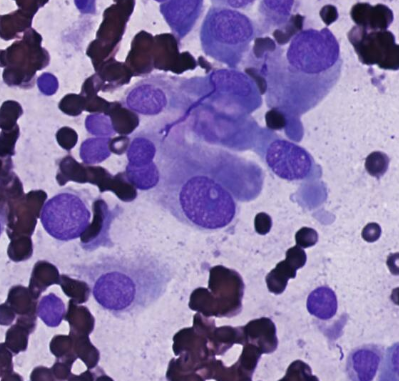
\includegraphics[scale=0.5]{image/inclusion_1.png}}
	\subfigure{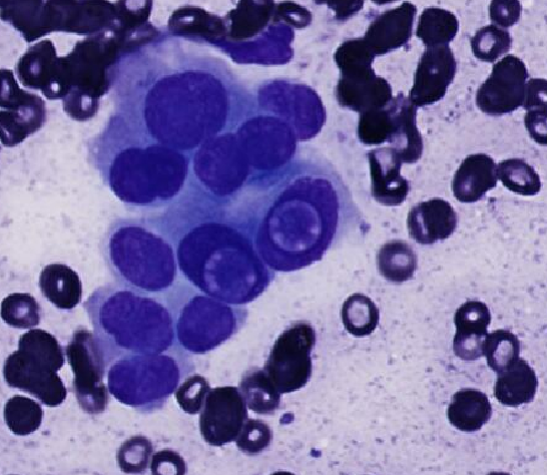
\includegraphics[scale=0.5]{image/inclusion_2.png}}
	\caption{Cells with inclusion}
	\label{fig:intro_inclu_ex}
\end{figure}

\begin{figure}
	\center
	\subfigure[Proliferative]{
		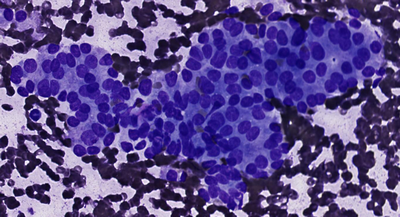
\includegraphics[scale=0.5]{image/prolif_pattern_1.png}
		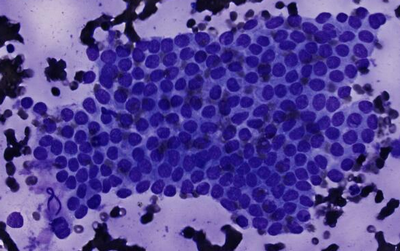
\includegraphics[scale=0.5]{image/prolif_pattern_2.png}
		\label{sfig:prolif_patterns}
	} \\
	\subfigure[Non-proliferative]{
		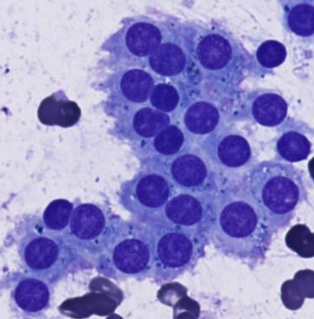
\includegraphics[scale=0.5]{image/normal_pattern_1.png}
		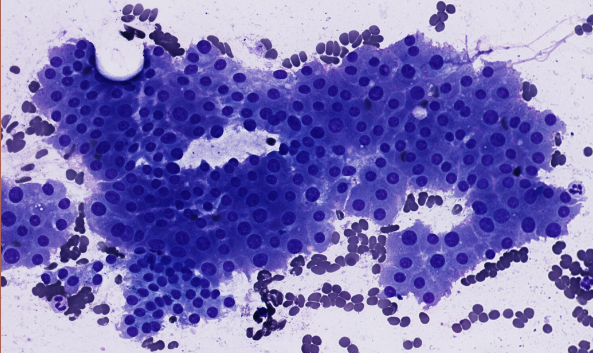
\includegraphics[scale=0.5]{image/normal_pattern_2.png}
		\label{sfig:norm_patterns}
	}
	\caption{Stained thyroid takings - architectural patterns}
	\label{fig:intro_pattern_ex}
\end{figure}


\subsubsection{Dataset}
\label{sssec:detection_thyroid_dataset}
A project dedicated to nodule malignancy detection was created on the Cytomine platform. It contains 61 annotated images with sizes ranging from 4 gigapixels to 18 gigapixels. Those images contain a total of 5784 labelled annotations performed by experts from the ULB (?? ref ??). Those labels (or terms) link the annotation to cytological objects related to the nodule malignancy problem. The terms made available on Cytomine are organized in an ontology which is divided into three main subcategories:

\begin{itemize}
	\item \textbf{Architectural patterns} : includes proliferative and non-proliferative patterns but also an intermediate class for patterns which present minor signs of proliferation.
	\item \textbf{Nuclear features} : includes cells with inclusion, normal cells and some additional cell-related terms
	\item \textbf{Others} : includes artefacts, background but also poly nuclear cells, red blood cells,...
\end{itemize} 

The complete ontology can be found in Appendix \ref{app:ontology}. Among those available terms, the ones that matter the most in the context of nodule malignancy detection are the cells with inclusion and the proliferative architectural patterns (major or with minor sign). Those terms represent the positive classes of the problem. The distributions of terms are given in Figure \ref{fig:ontology_histograms}. Those histograms highlight that a significant number of annotations have been made with the terms of interest. Moreover, the number of annotations is relatively balanced for those terms. While they are balanced taken alone, a problem arises when the terms are grouped. For instance, in the binary problem of determining whether a cell contains an inclusion or not, the positive class might be the term \textit{Cell with inclusion} while the negative class might contain the all the other terms from the cell subcategory (and possibly terms from the others subcategory). While being sound, this distribution of terms in both classes results in an imbalance which can be problematic when applying machine learning classification algorithms. The classes distribution for this example problem are given in Figure \ref{fig:imbalance_incl_vs_norm}.


\begin{figure}
	\center
	\subfigure[Main categories]{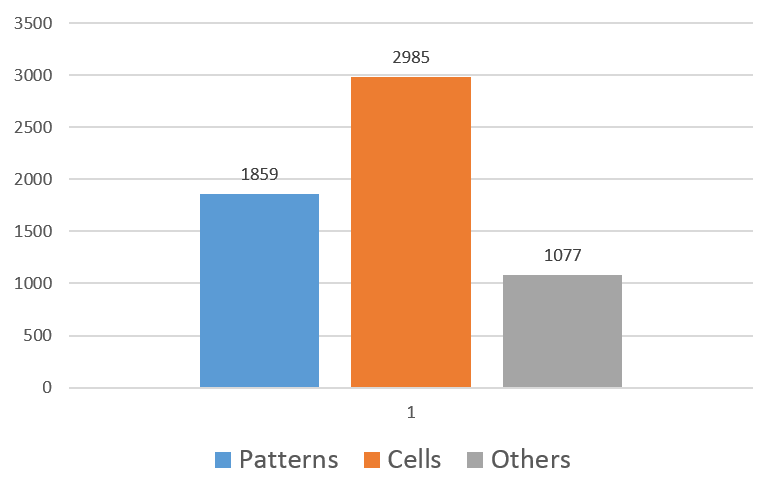
\includegraphics[scale=0.5]{image/ontology_hist_all.png}}
	\subfigure[Cell-related terms]{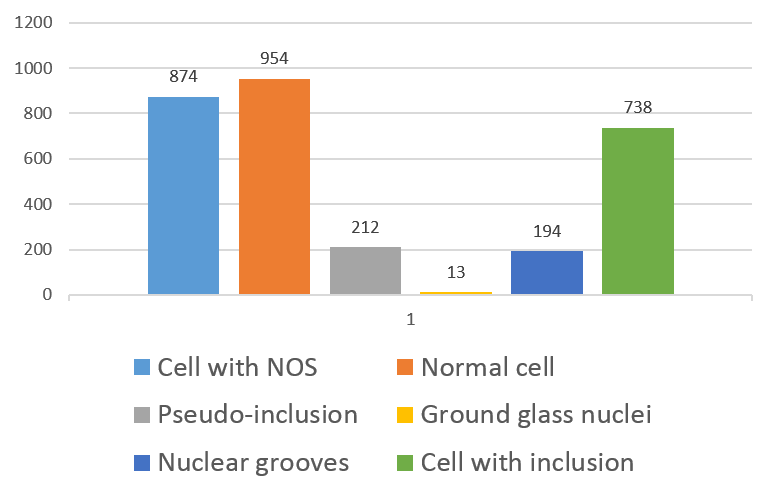
\includegraphics[scale=0.5]{image/ontology_hist_cells.png}}\\
	\subfigure[Pattern-related terms]{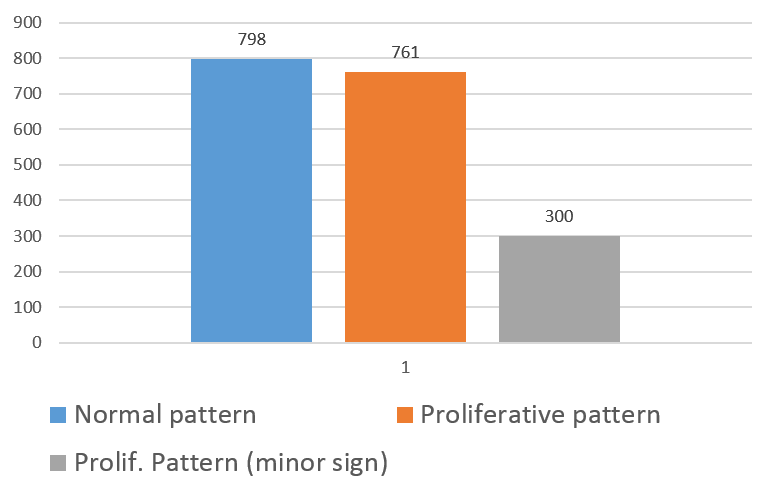
\includegraphics[scale=0.5]{image/ontology_hist_patterns.png}}
	\subfigure[Other terms]{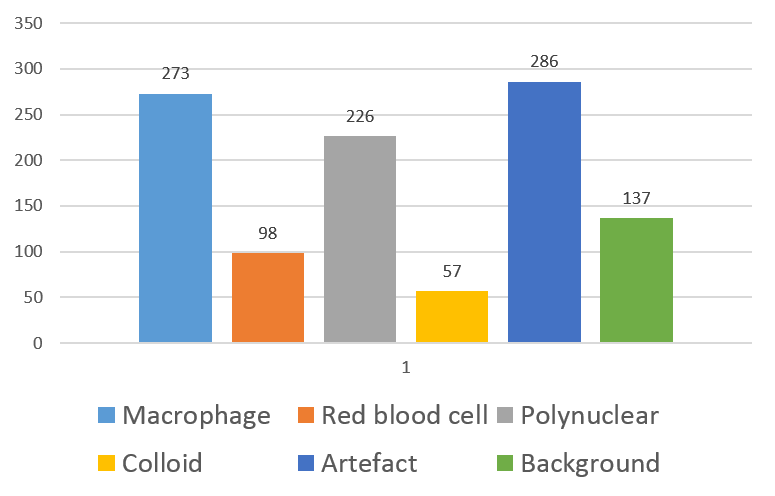
\includegraphics[scale=0.5]{image/ontology_hist_others.png}}
	\caption{Terms of the thyroid ontology - annotation counts histograms}
	\label{fig:ontology_histograms}
\end{figure}

\begin{figure}
	\center
	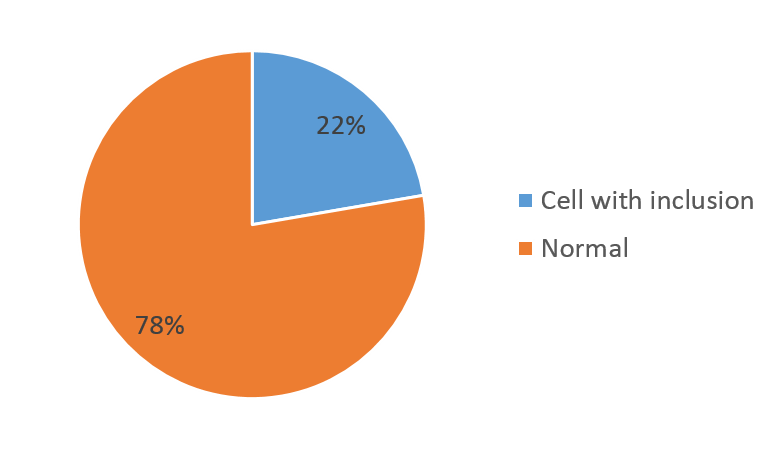
\includegraphics[scale=0.75]{image/imbalance_binary_problem.png}
	\caption{Cell inclusion detection problem. Terms in positive class: cell with inclusion. Terms in negative class: normal cells, pseudo inclusion, ground glass nuclei, nuclear grooves, red blood cells and poly-nuclear.}
	\label{fig:imbalance_incl_vs_norm}
\end{figure}